\documentclass[12pt]{article}
% \documentclass[a4paper,12pt]{article}
\usepackage[T1]{fontenc}
\usepackage[utf8]{inputenc}
\usepackage[polish]{babel}
\usepackage{graphicx}
\usepackage{amsfonts}
\usepackage{amsmath}
\usepackage{amssymb}
\usepackage{float}
\usepackage{booktabs}
\usepackage{hyperref}
\usepackage{listings}
\usepackage{caption}
\usepackage{subcaption}
\usepackage{parskip} 
\usepackage{geometry}
\usepackage[font=small, labelfont=bf]{caption}

\geometry{
    a4paper,
    top=2.5cm,
    bottom=2.5cm,
    left=2.5cm,
    right=2.5cm
}

% Styl dla kodu Python
\lstset{
    language=Python,
    basicstyle=\ttfamily\small,
    keywordstyle=\color{blue},
    commentstyle=\color{gray},
    stringstyle=\color{orange},
    breaklines=true,
    frame=single
}

\setlength{\textheight}{21cm}

\graphicspath{{figures/}}

\begin{document}

% ==================== STRONA TYTUŁOWA ====================
\begin{titlepage}
    \centering
    \vspace*{2cm}
    {\Large Zadanie nr 2 --- Próbkowanie i kwantyzacja \par}
    \vspace{0.5cm}
    {\large Cyfrowe Przetwarzanie Sygnałów \par}
    \vspace{2cm}
    {\large Ireneusz Bartoszek, 251481 \par}
    \vspace{0.5cm}
    {\large \today \par}
\end{titlepage}

% ==================== 1. CEL ZADANIA ====================
\section{Cel zadania}

Celem ćwiczenia było zapoznanie się z praktycznymi aspektami procesu konwersji
analogowo-cyfrowej (A/C) i cyfrowo-analogowej (C/A) sygnałów.
W ramach realizacji zadania zaimplementowano:
próbkowanie równomierne (S1),
kwantyzację równomierną z zaokrąglaniem (Q2),
rekonstrukcję metodą ekstrapolacji zerowego rzędu ZOH (R1)
oraz rekonstrukcję w oparciu o funkcję sinc (R3).
Zaimplementowano również miary podobieństwa sygnałów: MSE, SNR, PSNR oraz MD,
a także zademonstrowano zjawisko aliasingu dla trzech przypadków (A1, A2, A3).

% ==================== 2. WSTĘP TEORETYCZNY ====================
\section{Wstęp teoretyczny}

\subsection{Próbkowanie i twierdzenie Nyquista}

Próbkowanie polega na zamianie sygnału analogowego $x(t)$ na sygnał dyskretny
poprzez pobieranie wartości sygnału w równomiernie rozmieszczonych chwilach czasowych:
\begin{equation}
    x(n) = x(nT_s)
\end{equation}
gdzie $T_s = 1/f_s$ jest okresem próbkowania, a $f_s$ częstotliwością próbkowania.
Zgodnie z twierdzeniem Nyquista-Shannona, aby możliwe było wierne odtworzenie sygnału,
częstotliwość próbkowania musi być co najmniej dwukrotnie wyższa niż najwyższa
częstotliwość składowej sygnału \cite{instrukcja do zadania}.

\subsection{Kwantyzacja}

Kwantyzacja jest procesem odwzorowania amplitudy sygnału w skończony zbiór poziomów.
Przy $b$-bitowej reprezentacji liczba poziomów wynosi $2^b$, a próg kwantyzacji:
\begin{equation}
    \Delta = \frac{x_{max} - x_{min}}{2^b}
\end{equation}
Zastosowana metoda Q2 (zaokrąglanie) przypisuje każdej próbce wartość
najbliższego poziomu kwantyzacji. Błąd kwantyzacji można interpretować jako
addytywny szum. Dla sinusoidy idealny przetwornik $b$-bitowy charakteryzuje się:
\begin{equation}
    \text{SNR}_{A/C} \approx 6{,}02b + 1{,}76 \text{ dB}
\end{equation}
Efektywna liczba bitów (ENOB) rzeczywistego przetwornika:
\begin{equation}
    \text{ENOB} = \frac{\text{SNR} - 1{,}76}{6{,}02}
\end{equation}

\subsection{Rekonstrukcja sygnału}

Metoda ZOH (ekstrapolacja zerowego rzędu) przechowuje wartość próbki
aż do nadejścia kolejnej, tworząc charakterystyczny efekt schodkowy.
Metoda sinc opiera się na wzorze interpolacyjnym \cite{instrukcja do zadania}:
\begin{equation}
    x(t) = \sum_{n=-\infty}^{\infty} x(nT_s) \cdot \text{sinc}\!\left(\frac{t}{T_s} - n\right)
\end{equation}
gdzie znormalizowana funkcja sinc zdefiniowana jest jako:
\begin{equation}
    \text{sinc}(t) =
    \begin{cases}
        \dfrac{\sin(\pi t)}{\pi t} & \text{dla } t \neq 0 \\[6pt]
        1 & \text{dla } t = 0
    \end{cases}
\end{equation}
W praktycznej realizacji sumowanie ograniczono do $N_L$ próbek z lewej
i $N_R$ próbek z prawej strony punktu interpolacji.

\subsection{Miary podobieństwa sygnałów}

Do oceny jakości rekonstrukcji zastosowano następujące miary:
\begin{align}
    \text{MSE} &= \frac{1}{N} \sum_{i=0}^{N-1} \left[x(i) - \hat{x}(i)\right]^2 \\[4pt]
    \text{SNR}_{\text{dB}} &= 10 \log_{10} \frac{\sum_{i=0}^{N-1} x^2(i)}
                                                {\sum_{i=0}^{N-1} \left[x(i) - \hat{x}(i)\right]^2} \\[4pt]
    \text{PSNR}_{\text{dB}} &= 10 \log_{10} \frac{\max_i x(i)^2}{\text{MSE}} \\[4pt]
    \text{MD} &= \max_{i=0,\ldots,N} \left|x(i) - \hat{x}(i)\right|
\end{align}

\subsection{Aliasing}

Zjawisko aliasingu występuje gdy sygnał zawiera składową o częstotliwości $f_d$
wyższej niż połowa częstotliwości próbkowania $f_s/2$ (częstotliwość Nyquista).
Niemożliwe jest wówczas odróżnienie sygnału o częstotliwości $f_0$ od sygnału
o częstotliwości:
\begin{equation}
    f_d = f_0 + k \cdot f_s, \quad k \in \mathbb{Z}
\end{equation}

% ==================== 3. EKSPERYMENTY I WYNIKI ====================
\section{Eksperymenty i wyniki}

% -------------------- 3.1 Próbkowanie i rekonstrukcja --------------------
\subsection{Próbkowanie i rekonstrukcja}
\label{subsection:probkowanie_kwantyzacja}

\subsubsection{Założenia}

Wartości parametrów sygnału:
\begin{itemize}
    \item typ sygnału: sinusoidalny,
    \item amplituda ($A$): $2.0$,
    \item okres ($T$): $2.0$ s
    \item czas trwania ($d$): $10.0$ s
    \item częstotliwosc próbkowania ($f_{gen}$): $100.0$ Hz.
    % \item częstotliwość próbkowania referencyjna (pseudo-ciągła): $f_{ref} = 100$ Hz
\end{itemize}

Badano wpływ częstotliwości próbkowania ($f_s$) i metody rekonstrukcji (ZOH, sinc) na jakość odtworzonego sygnału

\subsubsection{Przebieg}

\begin{figure}[H]
    \centering
    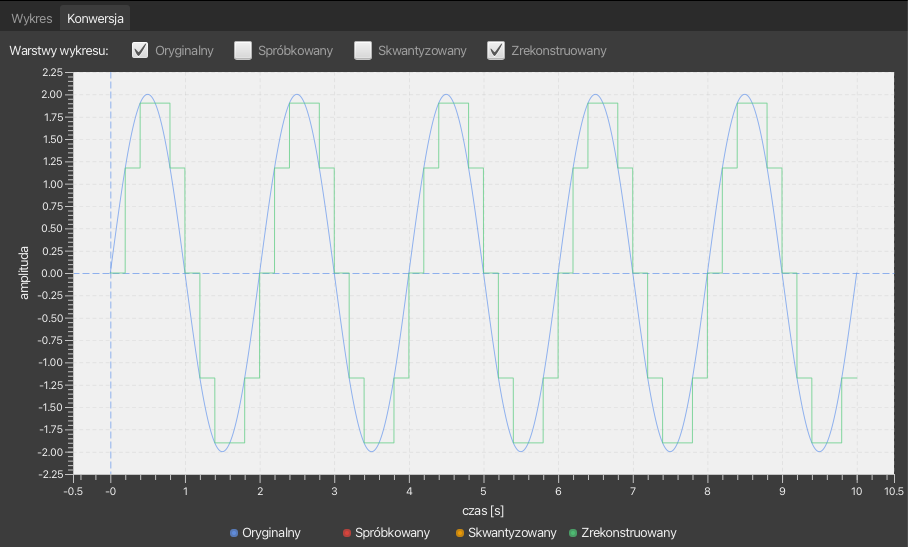
\includegraphics[width=0.85\textwidth]{reconstruction-zoh.png}
    \caption{Rekonstrukcja metodą ZOH --- sygnał oryginalny (niebieski)
             i zrekonstruowany (zielony). $f_s = 10$ Hz.}
    \label{fig:zoh}
\end{figure}

\begin{figure}[H]
    \centering
    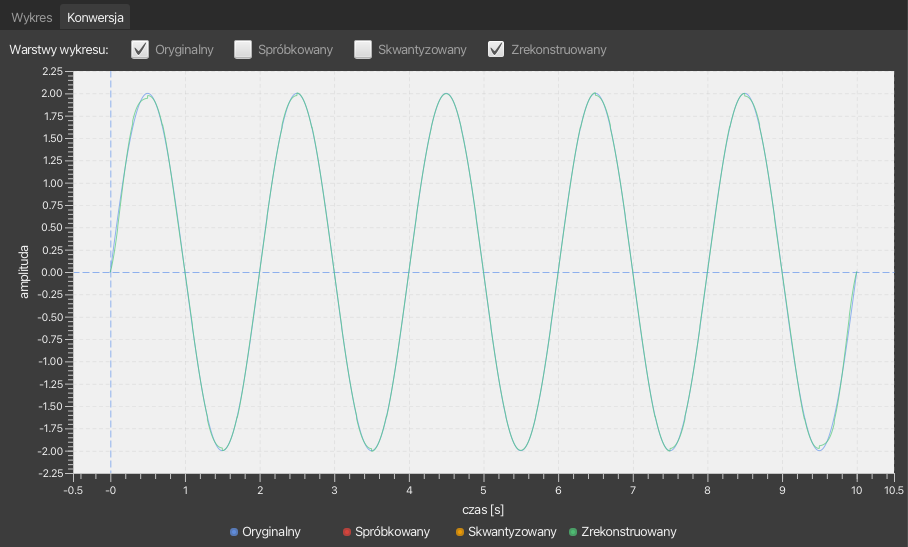
\includegraphics[width=0.85\textwidth]{reconstruction-sinc-20.png}
    \caption{Rekonstrukcja metodą sinc ($N_L = N_R = 20$) ---
             sygnał oryginalny (niebieski) i zrekonstruowany (zielony). $f_s = 5$ Hz.}
    \label{fig:sinc}
\end{figure}

\subsubsection{Rezultaty}

\begin{table}[H]
    \centering
    \caption{Miary podobieństwa dla różnych metod rekonstrukcji ($f_s = 5$ Hz)}
    \begin{tabular}{lcccc}
        \toprule
        \textbf{Metoda} & \textbf{MSE} & \textbf{SNR [dB]} & \textbf{PSNR [dB]} & \textbf{MD} \\
        \midrule
        \textbf{ZOH}              & 0.257638 & 8.90  & 11.91 & 1.175571 \\
        \textbf{sinc ($N=5$)}     & 0.000913 & 33.41 & 36.42 & 0.141894 \\
        \textbf{sinc ($N=10$)}    & 0.000583 & 35.35 & 38.36 & 0.130959 \\
        \textbf{sinc ($N=20$)}    & 0.000495 & 36.06 & 39.07 & 0.125716 \\
        \bottomrule
    \end{tabular}
    \label{tab:reconstruction}
\end{table}

Jak widać z Tab.~\ref{tab:reconstruction}, metoda sinc znacznie przewyższa metodę ZOH
pod względem wszystkich miar podobieństwa. Wartość MSE dla ZOH wynosi $0.258$,
podczas gdy dla sinc z $N=20$ jest ona ponad 500-krotnie mniejsza i wynosi $0.000495$.
Odpowiednio SNR wzrasta z $8.90$ dB dla ZOH do $36.06$ dB dla sinc z $N=20$.
Zwiększanie liczby próbek wykorzystywanych w interpolacji sinc poprawia jakość rekonstrukcji,
jednak korzyści maleją wraz ze wzrostem $N$ --- różnica między $N=10$ a $N=20$
jest znacznie mniejsza niż między $N=5$ a $N=10$.

% -------------------- 3.2 Kwantyzacja --------------------
\subsection{Kwantyzacja}

\subsubsection{Założenia}

Eksperyment przeprowadzono na tym samym sygnale sinusoidalnym (Podsekcja \ref{subsection:probkowanie_kwantyzacja}),
próbkowanym z $f_s = 20$ Hz. Badano wpływ liczby bitów kwantyzacji
na jakość sygnału skwantyzowanego.

\subsubsection{Przebieg}

\begin{figure}[H]
    \centering
    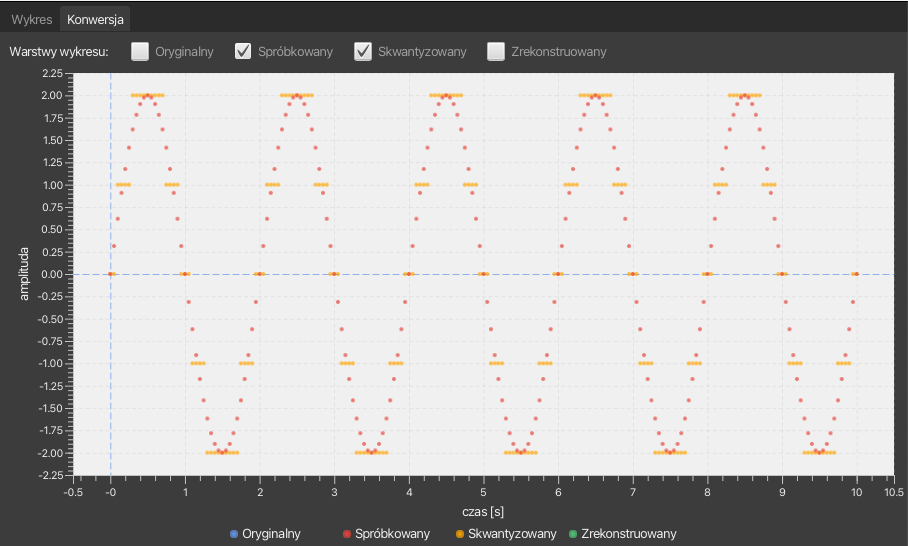
\includegraphics[width=0.85\textwidth]{figures/quantization-2.png}
    \caption{Kwantyzacja z zaokrąglaniem --- sygnał spróbkowany (niebieski)
             i skwantyzowany (pomarańczowy). Liczba bitów $b = 2$.}
    \label{fig:quantization-2}
\end{figure}

\begin{figure}[H]
    \centering
    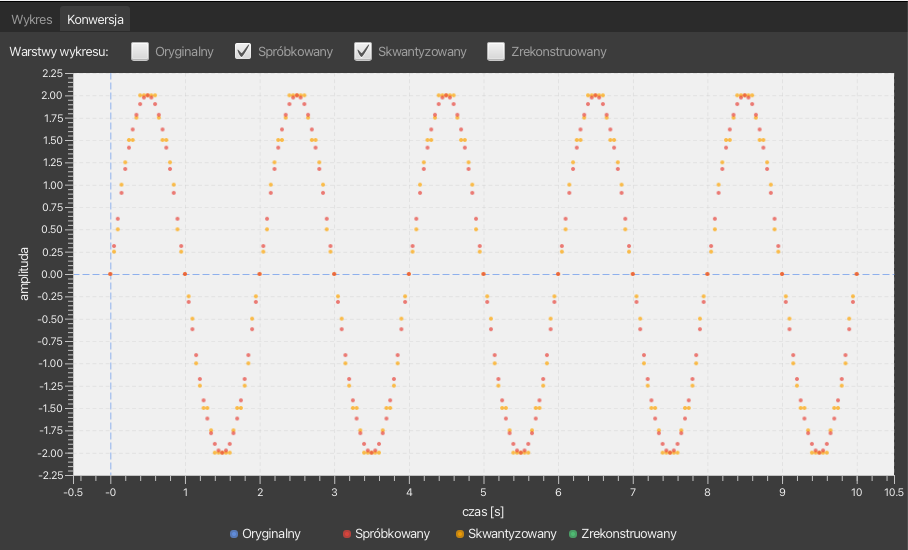
\includegraphics[width=0.85\textwidth]{figures/quantization-4.png}
    \caption{Kwantyzacja z zaokrąglaniem --- sygnał spróbkowany (niebieski)
             i skwantyzowany (pomarańczowy). Liczba bitów $b = 4$.}
    \label{fig:quantization-4}
\end{figure}

\begin{figure}[H]
    \centering
    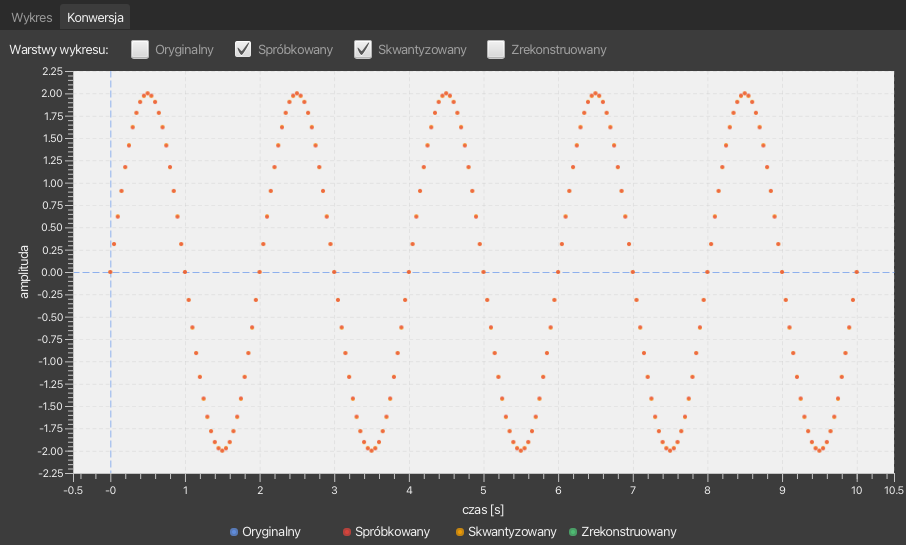
\includegraphics[width=0.85\textwidth]{figures/quantization-8.png}
    \caption{Kwantyzacja z zaokrąglaniem --- sygnał spróbkowany (niebieski)
             i skwantyzowany (pomarańczowy). Liczba bitów $b = 8$.}
    \label{fig:quantization-8}
\end{figure}

\subsubsection{Rezultaty}

\begin{table}[H]
    \centering
    \caption{Miary podobieństwa dla różnej liczby bitów kwantyzacji ($f_s = 20$ Hz)}
    \begin{tabular}{ccccccc}
        \toprule
        \textbf{Bity} & \textbf{Poziomy} & \textbf{MSE} & \textbf{SNR [dB]} & \textbf{SNR\textsubscript{teor} [dB]} & \textbf{PSNR [dB]} & \textbf{MD} \\
        \midrule
        2 & 4   & 0.065498 & 14.83 & 13.80 & 17.86 & 0.414214 \\
        4 & 16  & 0.006408 & 24.92 & 25.84 & 27.95 & 0.118034 \\
        8 & 256 & 0.000023 & 49.32 & 49.92 & 52.35 & 0.007661 \\
        \bottomrule
    \end{tabular}
    \label{tab:quantization}
\end{table}

Jak widać z Tab.~\ref{tab:quantization}, wraz ze wzrostem liczby bitów kwantyzacji
jakość sygnału skwantyzowanego znacznie się poprawia. Każde podwojenie liczby bitów
(dodanie jednego bitu) przekłada się na wzrost SNR o około $6$ dB, co jest zgodne
z teoretyczną zależnością $\text{SNR}_\text{teor} = 6{,}02b + 1{,}76$ dB.
Wartości zmierzone są zbliżone do teoretycznych --- największa rozbieżność
wynosi około $1$ dB dla $b=2$.
Obliczona wartość ENOB dla $b=8$ wynosi
$\text{ENOB} = (49{,}32 - 1{,}76) / 6{,}02 \approx 7{,}90$ bitów.

% -------------------- 3.3 Aliasing A1 --------------------
\subsection{Aliasing --- przypadek A1}

\subsubsection{Założenia}

\begin{itemize}
    \item Częstotliwość generowanego sygnału: $f_d = 1100$ Hz (Okres $T = 1/f_d \approx 0{,}000909$ s)
    \item Częstotliwość próbkowania: $f_s = 1000$ Hz
    \item Oczekiwana częstotliwość aliasu: $f_0 = f_d - f_s = 100$ Hz
    \item Badane amplitudy sygnału: $A \in \{0{,}5;\ 1{,}0;\ 2{,}0\}$
    \item Metoda rekonstrukcji: $\text{sinc}$, $N_L = N_R = 10$
\end{itemize}

\subsubsection{Przebieg}

\begin{figure}[H]
    \centering
    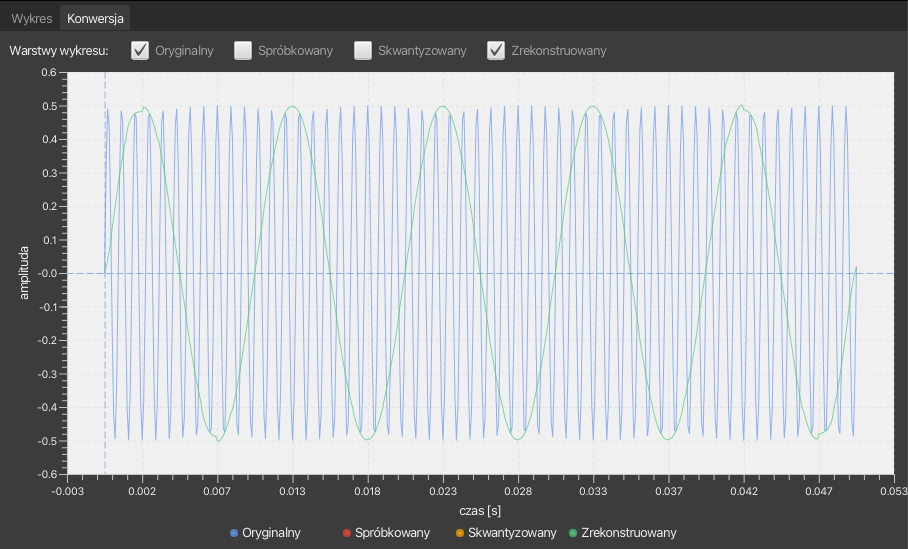
\includegraphics[width=0.85\textwidth]{A1-0_5.png}
    \caption{Aliasing A1 --- $f_d = 1100$ Hz, $A_d = 0.5$.
             Zrekonstruowany sygnał (zielony) ma częstotliwość $f_0 = 100$ Hz.}
    \label{fig:aliasing_a1_05}
\end{figure}

\begin{figure}[H]
    \centering
    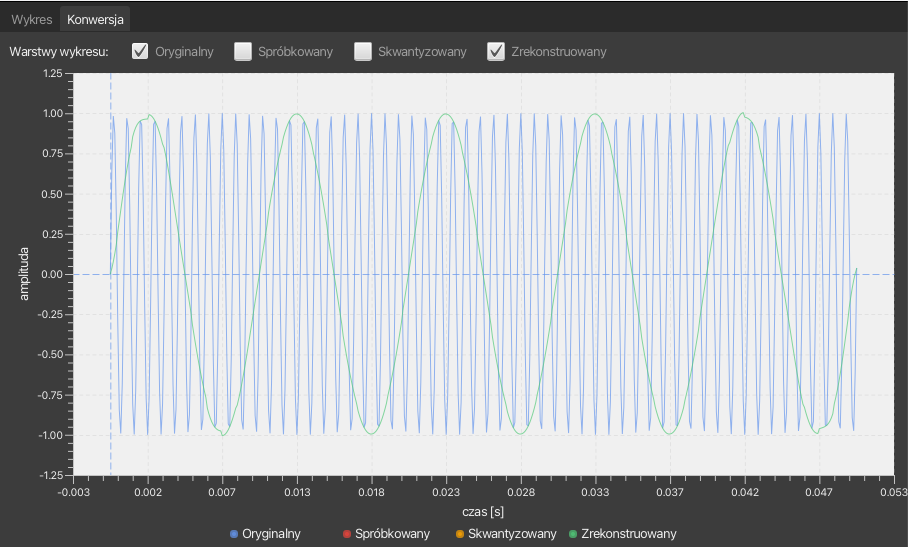
\includegraphics[width=0.85\textwidth]{figures/A1-1.png}
    \caption{Aliasing A1 --- $f_d = 1100$ Hz, $A_d = 1.0$.}
    \label{fig:aliasing_a1_10}
\end{figure}

\begin{figure}[H]
    \centering
    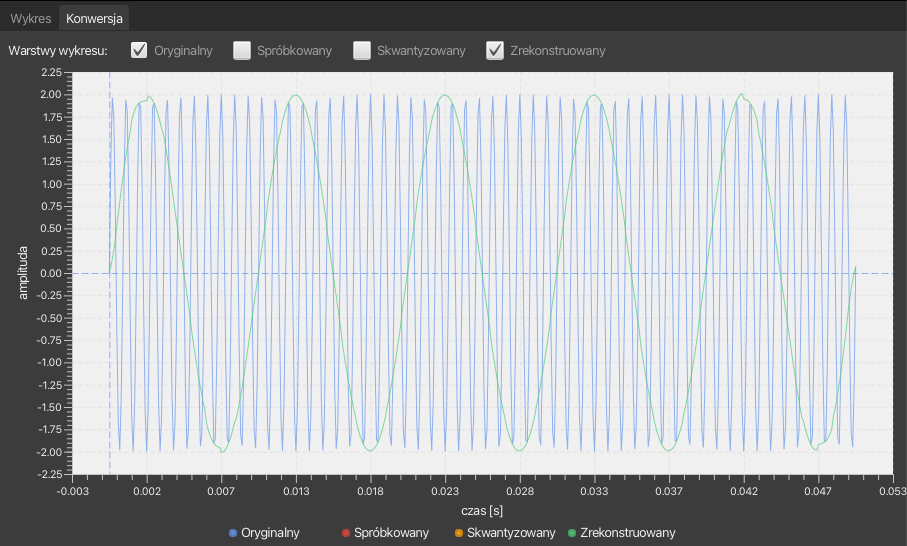
\includegraphics[width=0.85\textwidth]{figures/A1-2.png}
    \caption{Aliasing A1 --- $f_d = 1100$ Hz, $A_d = 2.0$.}
    \label{fig:aliasing_a1_20}
\end{figure}

\subsubsection{Rezultaty}

Jak widać z Rys.~\ref{fig:aliasing_a1_05}--\ref{fig:aliasing_a1_20},
sygnał o częstotliwości $f_d = 1100$ Hz po próbkowaniu z $f_s = 1000$ Hz
rekonstruuje się jako sygnał o częstotliwości $f_0 = 100$ Hz,
co jest zgodne z teoretyczną zależnością $f_d = f_0 + k \cdot f_s$.
Wartość SNR = $-3{,}01$ dB dla wszystkich amplitud potwierdza,
że zrekonstruowany sygnał znacznie różni się od oryginalnego $f_d$.
Wraz ze wzrostem amplitudy $A_d$ rośnie amplituda zrekonstruowanego sygnału
--- aliasing zachowuje proporcje amplitudy.

% -------------------- 3.4 Aliasing A2 --------------------
\subsection{Aliasing --- przypadek A2}

\subsubsection{Założenia}

\begin{itemize}
    \item Częstotliwość sygnału użytecznego (alias): $f_0 = 440$ Hz
    \item Częstotliwość próbkowania: $f_s = 22050$ Hz
    \item Częstotliwość sygnału powodującego aliasing: $f_d = f_0 + f_s = 22490$ Hz, okres $T_d = 1/f_d \approx 0{,}00004446$ s
    \item Częstotliwość generowania sygnału wejściowego: $f_{gen} = 220500$ Hz
    \item Badane amplitudy sygnału $f_d$: $A \in \{0{,}5;\ 1{,}0;\ 2{,}0\}$
    \item Metoda rekonstrukcji: $\text{sinc}$, $N_L = N_R = 10$
\end{itemize}

\subsubsection{Przebieg}

\begin{figure}[H]
    \centering
    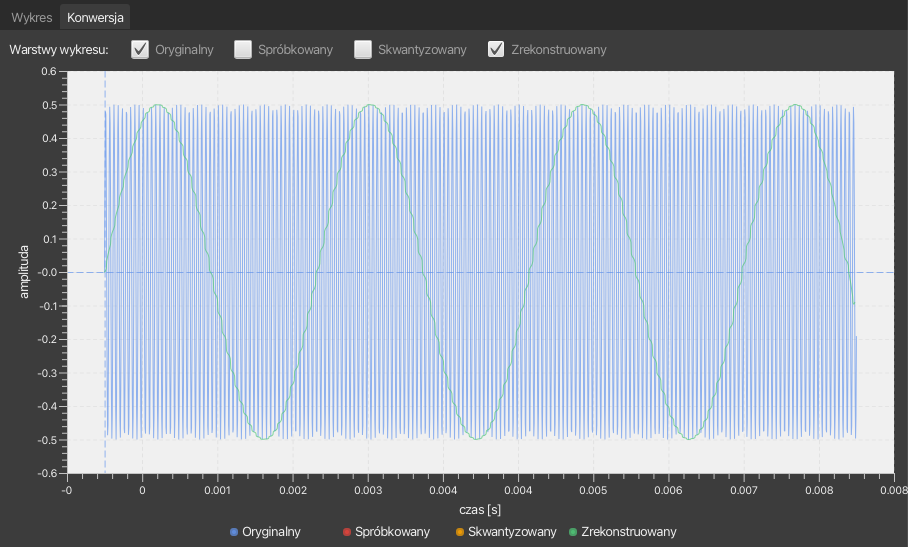
\includegraphics[width=0.85\textwidth]{A2-0_5.png}
    \caption{Aliasing A2 --- $f_d = 22490$ Hz, $A = 0.5$.
             Zrekonstruowany sygnał (zielony) ma częstotliwość $f_0 \approx 440$ Hz.}
    \label{fig:aliasing_a2_05}
\end{figure}

\begin{figure}[H]
    \centering
    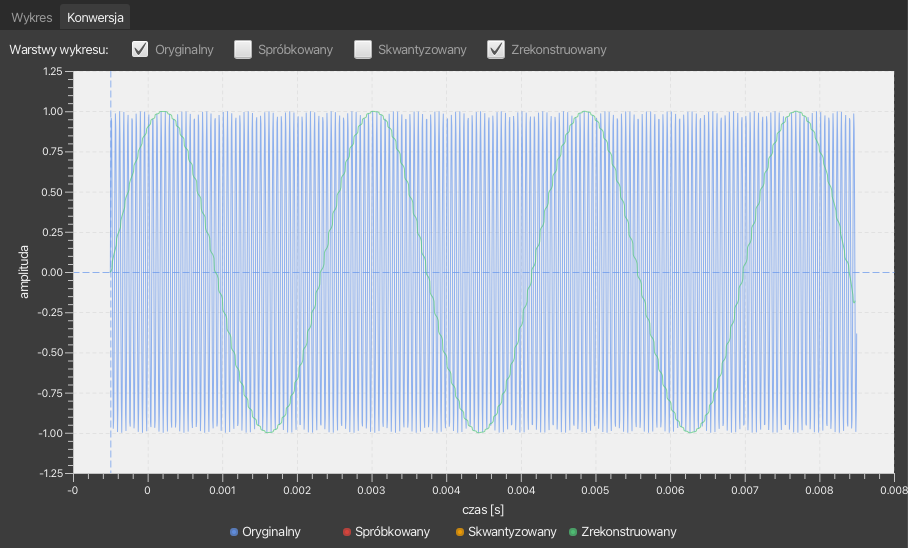
\includegraphics[width=0.85\textwidth]{A2-1_0.png}
    \caption{Aliasing A2 --- $f_d = 22490$ Hz, $A = 1.0$.}
    \label{fig:aliasing_a2_1}
\end{figure}

\begin{figure}[H]
    \centering
    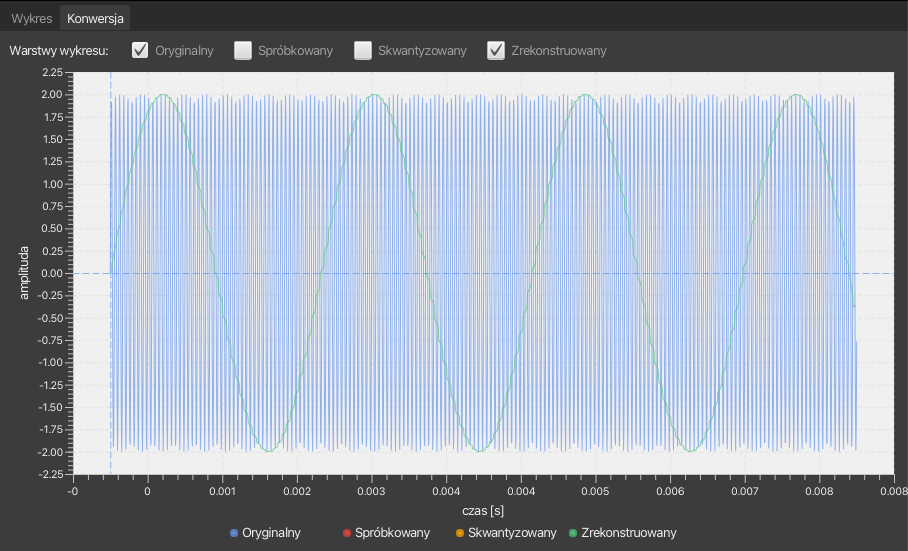
\includegraphics[width=0.85\textwidth]{A2-2_0.png}
    \caption{Aliasing A2 --- $f_d = 22490$ Hz, $A = 2.0$.}
    \label{fig:aliasing_a2_20}
\end{figure}


\subsubsection{Rezultaty}

Jak widać z Rys.~\ref{fig:aliasing_a2_05}--\ref{fig:aliasing_a2_20},
sygnał o częstotliwości $f_d = 22490$ Hz po próbkowaniu z $f_s = 22050$ Hz
rekonstruuje się jako sygnał o częstotliwości $f_0 \approx 440$ Hz,
co jest zgodne z zależnością $f_0 = f_d - f_s$.
Sygnał oryginalny (niebieski) jest tak wysokoczęstotliwościowy że na wykresie
wygląda jak wypełniony pas, natomiast zrekonstruowany alias (zielony)
ma wyraźnie widoczne okresy odpowiadające $f_0 = 440$ Hz.
Podobnie jak w przypadku A1, amplituda zrekonstruowanego sygnału
odpowiada amplitudzie sygnału wejściowego $f_d$.

% -------------------- 3.5 Aliasing A3 --------------------
\subsection{Aliasing --- przypadek A3}

\subsubsection{Założenia}

\begin{itemize}
    \item Częstotliwość sygnału użytecznego (alias): $f_0 = 220$ Hz
    \item Częstotliwość próbkowania: $f_s = 44100$ Hz
    \item Częstotliwość sygnału powodującego aliasing: $f_d = f_0 + f_s = 44320$ Hz, okres $T_d = 1/f_d \approx 0{,}00002256$ s
    \item Częstotliwość generowania sygnału wejściowego: $f_{gen} = 485100$ Hz
    \item Badane amplitudy sygnału $f_d$: $A \in \{0{,}5;\ 1{,}0;\ 2{,}0\}$
    \item Metoda rekonstrukcji: $\text{sinc}$, $N_L = N_R = 10$
\end{itemize}

\subsubsection{Przebieg}

\begin{figure}[H]
    \centering
    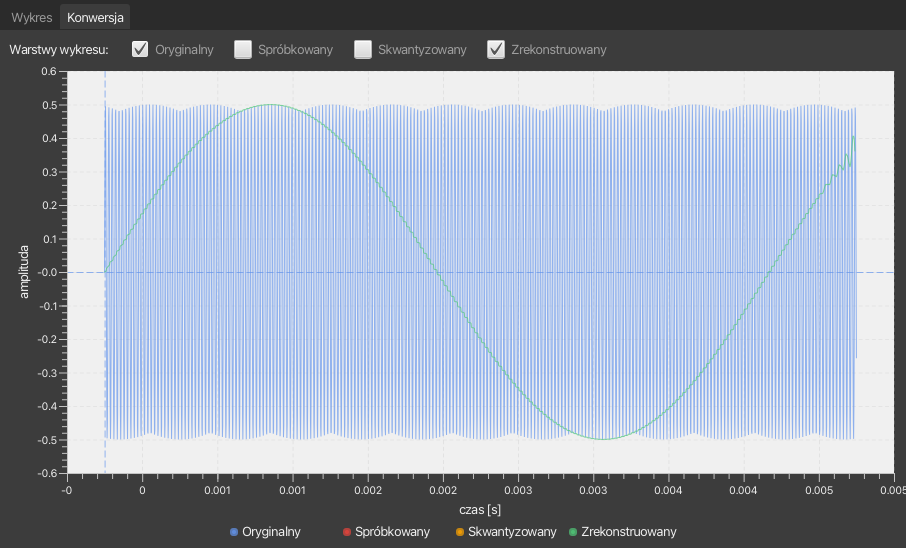
\includegraphics[width=0.85\textwidth]{A3-0_5.png}
    \caption{Aliasing A3 --- $f_d = 44320$ Hz, $A = 0.5$.
             Zrekonstruowany sygnał (zielony) ma częstotliwość $f_0 \approx 220$ Hz.}
    \label{fig:aliasing_a3_05}
\end{figure}

\begin{figure}[H]
    \centering
    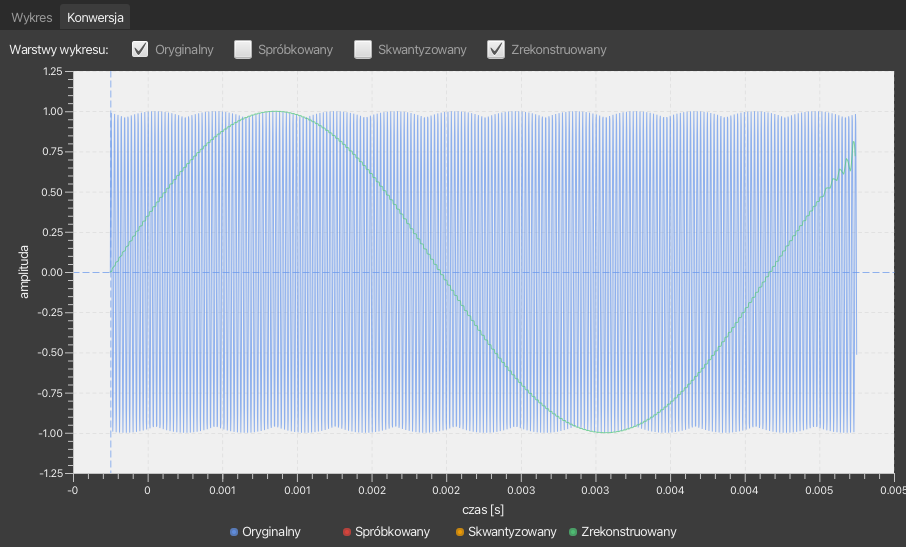
\includegraphics[width=0.85\textwidth]{A3-1.png}
    \caption{Aliasing A3 --- $f_d = 44320$ Hz, $A = 1.0$.}
    \label{fig:aliasing_a3_10}
\end{figure}

\begin{figure}[H]
    \centering
    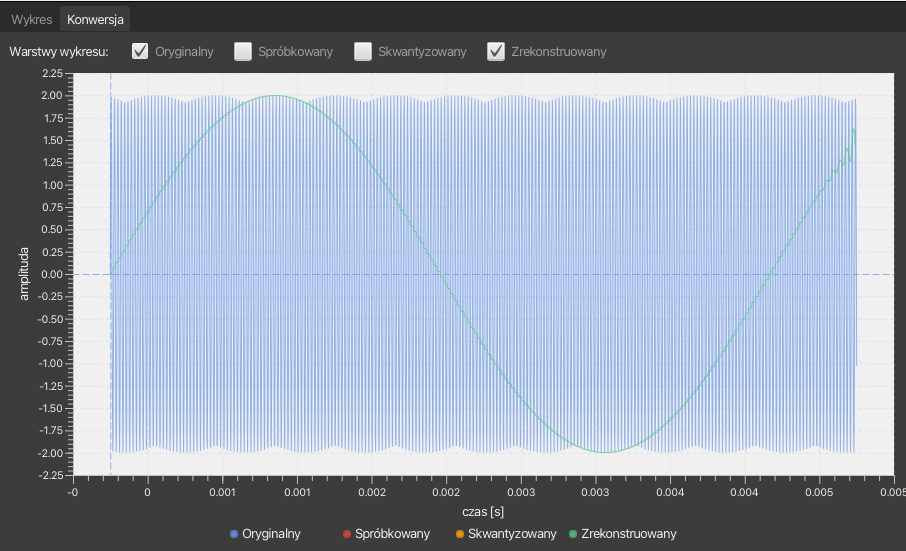
\includegraphics[width=0.85\textwidth]{A3-2.png}
    \caption{Aliasing A3 --- $f_d = 44320$ Hz, $A = 2.0$.}
    \label{fig:aliasing_a3_20}
\end{figure}

\subsubsection{Rezultaty}

Jak widać z Rys.~\ref{fig:aliasing_a3_05}--\ref{fig:aliasing_a3_20},
sygnał o częstotliwości $f_d = 44320$ Hz po próbkowaniu z $f_s = 44100$ Hz
rekonstruuje się jako sygnał o częstotliwości $f_0 \approx 220$ Hz,
co jest zgodne z zależnością $f_0 = f_d - f_s$.
Wyniki są analogiczne do przypadków A1 i A2 ---
amplituda zrekonstruowanego sygnału odpowiada amplitudzie sygnału wejściowego $f_d$,
a częstotliwość aliasu wynosi $f_0 = f_d - f_s = 44320 - 44100 = 220$ Hz.

% ==================== 4. WNIOSKI ====================
\section{Wnioski}

\begin{itemize}
    \item Metoda $\text{sinc}$ znacznie przewyższa ZOH pod względem jakości rekonstrukcji
    --- SNR wzrósł z $8.90$ dB (ZOH) do $36.06$ dB ($\text{sinc}$, $N=20$).
    Zwiększanie $N$ poprawia wyniki, lecz z malejącymi korzyściami.

    \item Każdy dodatkowy bit kwantyzacji przekłada się na wzrost SNR o około $6$ dB,
    zgodnie z zależnością $\text{SNR}_\text{teor} = 6.02b + 1.76$ dB.
    Dla $b=8$ obliczone ENOB wyniosło $7.90$.

    \item We wszystkich przypadkach (A1, A2, A3) zademonstrowano aliasing ---
    sygnał o $f_d > f_s/2$ rekonstruuje się jako sygnał o $f_0 = f_d - f_s$.
    Amplituda aliasu odpowiada amplitudzie sygnału wejściowego.
\end{itemize}

% ==================== BIBLIOGRAFIA ====================
\begin{thebibliography}{9}

\bibitem{instrukcja do zadania} Instrukcja "Zadanie 2 - Próbkowanie i kwantyzacja".

\end{thebibliography}

\end{document}
